
\subsection*{Reality.}


Following \citet{kriegman2019automated}, simulated voxels were realized physically as pneumatically actuated, hollow silicone voxels.
The physical robot in \cite{kriegman2019automated} was constructed to transfer symmetrical shape change, so its actuated voxels were distributed symmetrically and hooked into a single pressure inlet.
Thus, pressure oscillations occurred symmetrically in phase, and the robot could only pulse in place.
Moreover, due to thin voxel walls relative to overall voxel size, and the tubing and glue used to bond them together, the robot in \cite{kriegman2019automated} could not fully support its own weight.
The robot was lifted off the ground by placing it on top of a small petri dish, positioned underneath a segment of entirely passive voxels in the center of the robot's ventral surface.
This permitted ventral (and more extreme global) changes in surface curvature, yielding successful sim2real transfer of shape change, 
but not locomotion.


The construction kit presented here rectifies the weight issue by miniaturizing the voxels---voxel length was halved (from 3cm to 1.5cm) and the wall thickness remained the same (1mm), reducing voxel mass from 4.3g to 1.2g (including tubing but not pneumatic connectors).
Further, the inter-voxel tubing and glue was replaced with holes punched through the walls of adjacent active voxels in the same x,y slice, before attaching them with a shared bottom layer (Fig.~\ref{fig:real}d).
Finally, locomotion is now possible because separate contiguous sections of voxels in each slice can be arbitrarily actuated in or out of phase with other sections across the body.



\begin{figure}[t]
    \centering
    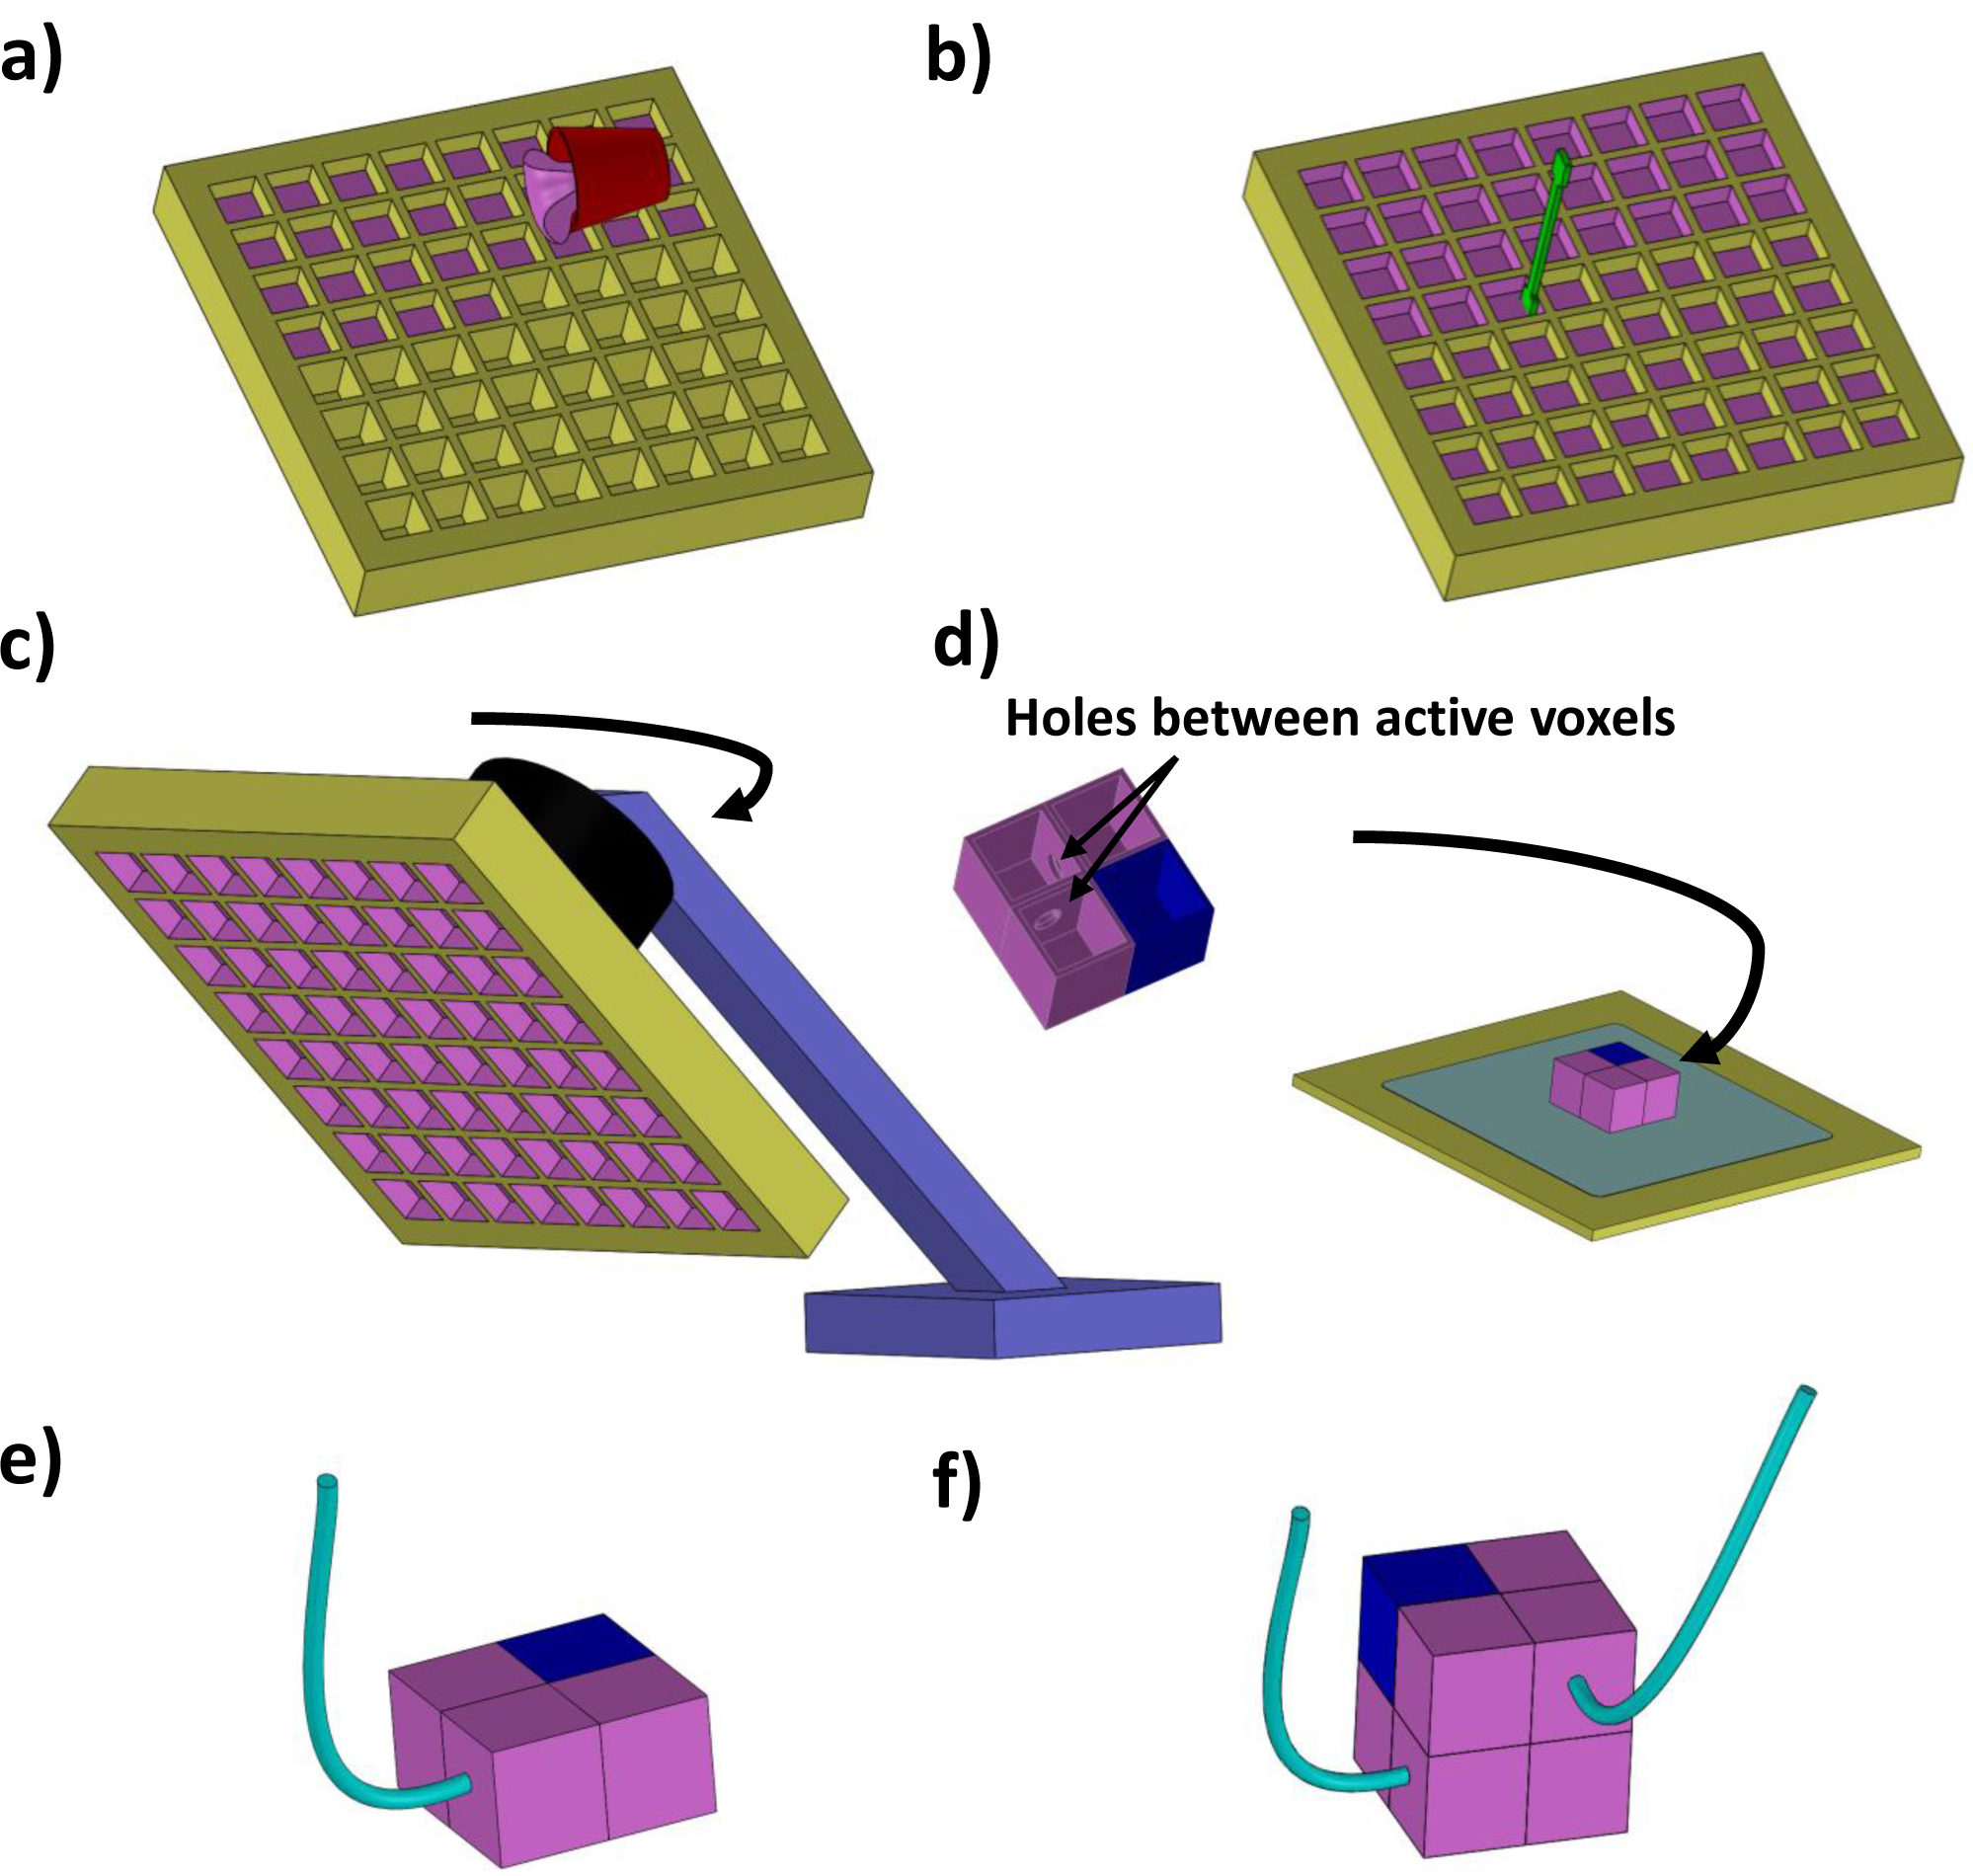
\includegraphics[width=0.7\linewidth]{Chapter02/fig/voxel_manufacturing.jpg}
    % \vspace{0pt}
    \caption{\textbf{Manufacturing modular soft robots.}
    Hollow, silicone voxels were created by partially filling an open-face mold with silicone (\textbf{a}), 
    using a spatula to spread it along the interior walls (\textbf{b}), and then securing the mold to a 1-axis rotational molding machine (\textbf{c}). This process allowed excess silicone to drip out of the mold, while spreading the remaining silicone into a thin uniform layer.
    The cured, bottomless voxels were then appropriately arranged and connected for each x,y slice of the design, and bonded with a shared bottom layer (\textbf{d}).
    Finally, tubing was attached (\textbf{e}), and the slices were stacked and bonded to form the design (\textbf{f}). 
    Video:
\href{https://youtu.be/jbQ2T7jIYRU}{\color{blue}\tt\textbf{youtu.be/jbQ2T7jIYRU}}.
    }
    \label{fig:real}
    % \vspace{-1.5em}
\end{figure}



\subsection*{The build protocol.}


The voxels were manufactured using a single-axis rotational molding machine.
First, an open-face mold was fabricated by interlacing 26 acrylic strips into a flat base, to form a lattice of cubic concavities, resembling an ice-cube tray (Fig.~\ref{fig:real}a). Mold components were laser-cut (VLS2.30, Universal Laser System) from a flat acrylic sheet with a thickness of 0.025 inch.
Next, silicone (Dragon Skin 10 Fast; Smooth-On, Inc.) was poured into the acrylic mold (Fig.~\ref{fig:real}a), and a spatula was used to spread the silicone along the interior walls of each cavity (Fig.~\ref{fig:real}b). Colored pigment was added to each batch of silicone to indicate whether the voxel was active or passive, simplifying the assembly process. Here we used pink for active voxels and blue or yellow for passive voxels.

The mold was then flipped upside down and secured to a 1-axis rotational molding machine. The machine was clamped to a table with binder clips, angled $45^{\circ}$ relative to horizontal, and set to rotate $90^{\circ}$ every 45 seconds (Fig.~\ref{fig:real}c).
This allowed the silicone to flow and evenly coat the walls of the mold, as excess silicone dripped out. 
After the voxels partially cured for 25 minutes at room temperature, the mold was moved to an incubator, with a temperature of $60^{\circ}$C for another 20 minutes. 
(Without an incubator, the silicone will take 75 minutes to fully cure at room temperature.)

The above steps were then repeated to add an additional layer of silicone.
Once the second layer cured, the bottomless voxels were removed from the mold using an X-Acto knife, and excess silicone around their edges was trimmed.

In the next step, each x,y slice (or dorsal plane) of the design was assembled by using Sil-Poxy (Smooth-On, Inc.) to bond adjacent voxels and prevent the slice from shifting.
Holes were then punched between adjacent active voxels so that contiguous collections of voxels could be actuated together in phase.
Each actuator group needed to contain at least one voxel on the surface of the design so that it could be controlled by an external pressure inlet.
To create the bottom layer, two 1mm-thick rulers were attached to an acrylic substrate using double-sided tape and silicone was poured in the space between them. 
Then, the slice of bottomless voxels was flipped, open-side down, onto this uncured silicone layer (Fig.~\ref{fig:real}d). 

After the bottom layer cured, a thin layer of silicone was applied with a popsicle stick along the outermost portions of the interstices of the voxels, bonding adjacent voxels (without gluing over inter-voxel holes).
Then, the slice was cut from the silicone sheet and a hole was poked into the side of one exterior voxel from each group of active voxels.
Next, a 1/32'' ID silicone tube was inserted into the hole, and glued in place with Sil-Poxy, applied with a Q-tip (Fig.~\ref{fig:real}e). 
The end of this tube was then connected to a straight pneumatic connector, which was connected to 1/16'' ID silicone tubing.

Occasional imperfections in alignment, silicone thickness, or inter-voxel hole sizes would result in leaky structures. 
Leaks were detected by filling a beaker with water, submerging the voxels, and inflating them. 
Bubbles would emanate from leaks, which were repaired with Sil-Poxy.
After repairing any leaks, the slices were stacked on top of each other and bonded together using a thin layer of silicone (Fig.~\ref{fig:real}e). 
Finally, these layers were connected pneumatically with assorted pneumatic connectors, attached to 1/16'' ID silicone tubes. 
